%%%%%%%%%%%%%%%%%%%%%%%%%%%%% Define Article %%%%%%%%%%%%%%%%%%%%%%%%%%%%%%%%%%
\documentclass[hidelinks,11pt]{article}
%%%%%%%%%%%%%%%%%%%%%%%%%%%%%%%%%%%%%%%%%%%%%%%%%%%%%%%%%%%%%%%%%%%%%%%%%%%%%%%

%%%%%%%%%%%%%%%%%%%%%%%%%%%%% Using Packages %%%%%%%%%%%%%%%%%%%%%%%%%%%%%%%%%%
\usepackage{geometry}
\usepackage{graphicx}
\usepackage{amssymb}
\usepackage{amsmath}
\usepackage{amsthm}
\usepackage{empheq}
\usepackage{url}
\usepackage{mdframed}
\usepackage{booktabs}
\usepackage{float}
\usepackage{lipsum}
\usepackage{graphicx}
\usepackage[french]{babel}
\usepackage{caption}
\usepackage{subcaption}
\usepackage{color}
\usepackage{psfrag}
\usepackage{pgfplots}
\usepackage{bm}
\usepackage{hyperref}
%%%%%%%%%%%%%%%%%%%%%%%%%%%%%%%%%%%%%%%%%%%%%%%%%%%%%%%%%%%%%%%%%%%%%%%%%%%%%%%

% Other Settings

%%%%%%%%%%%%%%%%%%%%%%%%%% Page Setting %%%%%%%%%%%%%%%%%%%%%%%%%%%%%%%%%%%%%%%
\geometry{a4paper}

%%%%%%%%%%%%%%%%%%%%%%%%%% Define some useful colors %%%%%%%%%%%%%%%%%%%%%%%%%%
\definecolor{ocre}{RGB}{243,102,25}
\definecolor{mygray}{RGB}{243,243,244}
\definecolor{deepGreen}{RGB}{26,111,0}
\definecolor{shallowGreen}{RGB}{235,255,255}
\definecolor{deepBlue}{RGB}{61,124,222}
\definecolor{shallowBlue}{RGB}{235,249,255}
%%%%%%%%%%%%%%%%%%%%%%%%%%%%%%%%%%%%%%%%%%%%%%%%%%%%%%%%%%%%%%%%%%%%%%%%%%%%%%%

%%%%%%%%%%%%%%%%%%%%%%%%%% Define an orangebox command %%%%%%%%%%%%%%%%%%%%%%%%
\newcommand\orangebox[1]{\fcolorbox{ocre}{mygray}{\hspace{1em}#1\hspace{1em}}}
%%%%%%%%%%%%%%%%%%%%%%%%%%%%%%%%%%%%%%%%%%%%%%%%%%%%%%%%%%%%%%%%%%%%%%%%%%%%%%%

%%%%%%%%%%%%%%%%%%%%%%%%%%%% English Environments %%%%%%%%%%%%%%%%%%%%%%%%%%%%%
\newtheoremstyle{mytheoremstyle}{3pt}{3pt}{\normalfont}{0cm}{\rmfamily\bfseries}{}{1em}{{\color{black}\thmname{#1}~\thmnumber{#2}}\thmnote{\,--\,#3}}
\newtheoremstyle{myproblemstyle}{3pt}{3pt}{\normalfont}{0cm}{\rmfamily\bfseries}{}{1em}{{\color{black}\thmname{#1}~\thmnumber{#2}}\thmnote{\,--\,#3}}
\theoremstyle{mytheoremstyle}
\newmdtheoremenv[linewidth=1pt,backgroundcolor=shallowGreen,linecolor=deepGreen,leftmargin=0pt,innerleftmargin=20pt,innerrightmargin=20pt,]{theorem}{Theorem}[section]
\theoremstyle{mytheoremstyle}
\newmdtheoremenv[linewidth=1pt,backgroundcolor=shallowBlue,linecolor=deepBlue,leftmargin=0pt,innerleftmargin=20pt,innerrightmargin=20pt,]{definition}{Definition}[section]
\theoremstyle{myproblemstyle}
\newmdtheoremenv[linecolor=black,leftmargin=0pt,innerleftmargin=10pt,innerrightmargin=10pt,]{problem}{Problem}[section]
%%%%%%%%%%%%%%%%%%%%%%%%%%%%%%%%%%%%%%%%%%%%%%%%%%%%%%%%%%%%%%%%%%%%%%%%%%%%%%%

%%%%%%%%%%%%%%%%%%%%%%%%%%%%%%% Plotting Settings %%%%%%%%%%%%%%%%%%%%%%%%%%%%%
\usepgfplotslibrary{colorbrewer}
\pgfplotsset{width=8cm,compat=1.9}
%%%%%%%%%%%%%%%%%%%%%%%%%%%%%%%%%%%%%%%%%%%%%%%%%%%%%%%%%%%%%%%%%%%%%%%%%%%%%%%

%%%%%%%%%%%%%%%%%%%%%%%%%%%%%%% Title & Author %%%%%%%%%%%%%%%%%%%%%%%%%%%%%%%%
\title{Rapport Projet IPT : Détection de contours dans une image}
\author{Charlotte Thomas \\ Naïs Baubry}
%%%%%%%%%%%%%%%%%%%%%%%%%%%%%%%%%%%%%%%%%%%%%%%%%%%%%%%%%%%%%%%%%%%%%%%%%%%%%%%

\begin{document}
    \maketitle
    \begin{abstract}
        De la reconnaissance faciale à la la médecine de pointe, de nombreuses applications modernes
        demandent de reconnaître les contours d'une image. C'est pour ces raisons que par ce projet,
        nous allons étudier une méthode matricielle de détection de contours dans une image : le filtre
        de Canny.
    \end{abstract}
    \tableofcontents
    \cleardoublepage
    
    \section{Détourer une image}
    \subsection{Solutions envisageables}
    En traitement d'images et en vision par ordinateur, on appelle détection de contours les procédés permettant de repérer
    les points d'une image matricielle qui correspondent à un changement brutal de l'intensité lumineuse. 
    Pour traiter ces images, plusieurs méthodes sont possibles :
    
    \begin{itemize}
        \item Le filtre de Roberts met en évidence la différence d'intensité en suivant les diagonales de l'image.
        \newline
        $\\\begin{pmatrix}
            0 & 0 & 0 \\
            0 & 0 & 1 \\
            0 & -1 & 0
        \end{pmatrix}$
        et $
            \begin{pmatrix}
                0 & 0 & 0 \\
                0 & -1 & 0 \\
                0 & 0 & 1
            \end{pmatrix}
        $
        \bigskip
        \item Le filtre de Prewitt met en évidence la différence d'intensité en suivant les axes verticaux et horizontaux.
        \newline
        $\\\dfrac{1}{3}\begin{pmatrix}
            -1 & 0 & 1 \\
            -1 & 0 & 1 \\
            -1 & 0 & 1
        \end{pmatrix}$
        et $
        \dfrac{1}{3}\begin{pmatrix}
                -1 & -1 & -1 \\
                0 & 0 & 0 \\
                1 & 1 & 1
            \end{pmatrix}
        $
        \bigskip
        \item Le filtre de Sobel utilise un principe assez semblable aux deux premiers filtres présentés, seul l’opérateur est modifié. 
        Le principal avantage des filtres de Sobel et Prewitt est leur facilité de mise en œuvre ainsi que la rapidité de leur traitement. 
        De plus, ils utilisent un opérateur de lissage qui améliore le rendu final. 
        Mais leur grande sensibilité au bruit les rends moins performant.
        \newline
        $\\\dfrac{1}{4}\begin{pmatrix}
            -1 & 0 & 1 \\
            -2 & 0 & 2 \\
            -1 & 0 & 1
        \end{pmatrix}$
        et  $ 
        \dfrac{1}{4}\begin{pmatrix}
                -1 & -2 & -1 \\
                0 & 0 & 0 \\
                1 & 2 & 1
            \end{pmatrix}
        $
        \bigskip
        \item Le filtre de Canny est une amélioration du filtre de Sobel et utilise un opérateur gaussien. Il suit trois critères: 
        \begin{enumerate}
            \item \textit{bonne détection :} faible taux d'erreur dans la signalisation des contours,
            \item \textit{bonne localisation :} minimisation des distances entre les contours détectés et les contours réels,
            \item \textit{clarté de la réponse :} une seule réponse par contour et pas de faux positifs.
        \end{enumerate}
    \end{itemize}
    Lors de ce projet, nous avons étudié plus particulièrement le filtre de Canny. 
    \begin{figure}
        \centering
        \includegraphics[width=0.5\textwidth]{figs/fig1}
        \caption{Différents résultats en fonction du filtre utilisé}
    \end{figure}


    \subsection{Algorithme de Canny \cite{canny}}

    L'algorithme de Canny permet de détecter les bordures d'une image, il est découpé en plusieurs phases
    \begin{enumerate}
        \item Un filtre gaussien de taille impaire et de paramètre sigma ( l’écart type )
         est appliqué sur la matrice de l’image pour réduire le bruit de l’image et améliorer la détection des contours : c’est l’étape de \textbf{\textit{bruit}}.
        \item On fait ensuite la convolution de la matrice de l’image et de deux matrices de gradient pour avoir le gradient en X et en Y de 
        la matrice ( prise comme une fonction de deux variables ), 
        ces deux matrices servent à calculer la matrice de gradient ( la norme du gradient ) 
        pour avoir une première approximation, c’est l’étape de \textit{\textbf{gradient}}.
        \item L’étape précédente fait des bordures plutôt grossières, alors ensuite on traite la matrice par bloc de 9 pixels 
        ( carré de 3 par 3 ) et on cherche les maximas locaux pour affiner l’image, c’est l’étape \textit{\textbf{d’affinage}}.
        \item Ensuite, on applique un seuillage ( avec deux paramètres haut et bas ). 
        L’algorithme de seuillage permet de mettre tous les pixels à 0 ou 1 basé sur s’ils sont sur une bordure ou non,
        afin d’obtenir un meilleur contraste, c’est l’étape de \textit{\textbf{seuillage}}.
    \end{enumerate}
    \begin{figure}[b]
        \centering
        \includegraphics[width=0.3\textwidth]{figs/fig2}
        \caption{Exemple d'une image passé par l'algorithme de Canny}
    \end{figure}

    \section{Implémentation}
    \subsection{Raffinage}
    Nous avons découpé au maximum le code afin qu’il soit lisible et agréable à maintenir. 
    \textit{N.B : les types renvoyés sont en \textbf{gras} et en italique} \newline

    \textit{\textbf{Fonctions de support : }} elles sont utilisées dans les 4 fonctions principales représentant les étapes de l'algorithme
    \newline
    \begin{itemize}
        \item \textit{image\textunderscore to\textunderscore array (finalename: str) $\rightarrow$ \textbf{np.array}} : transforme une image donnée en entrée (sous une forme de sa localisation ) en array numpy. 
        \smallskip
        \item \textit{superposition(i: int; j: int; tableau: np.array; masque: np.array) $\rightarrow$  \textbf{bool} }: renvoie si le masque peut être superposé centré en $(i,j)$. 
        \smallskip
        \item \textit{calcul(i: int, j: int, tableau: np.array; masque: np.array) $\rightarrow$  \textbf{float}} : renvoie l’indice $(i,j)$ de la convolution de $tableau$ par $masque$.
        \smallskip
        \item \textit{masque(image: np.array, mask: np.array, name=”Masque”: str, char=”\#”) $\rightarrow$  \textbf{np.array}} : renvoie la convolution $d’image$ par le tableau $mask$, avec une progressbar de titre masque.
        \smallskip
        \item \textit{gausse(x:int; y: int; sigma: float) : $\rightarrow$  \textbf{float}} : fonction de Gauss de paramètre sigma
        \smallskip
        \item \textit{voisin(i: int; j: int; image: np.array) $\rightarrow$  \textbf{bool} }: renvoie si le pixel $(i,j)$ a un voisin blanc
        \newline
    \end{itemize}
    
    \textit{\textbf{Fonctions principales : }} ce sont les 4 fonctions qui mettent en place les différentes étapes de l'algorithme
    \newline
    
    \begin{itemize}
        \item \textit{bruit(taille: int; sigma: float; image: np.array) $\rightarrow$ \textbf{np.array} }: calcule le masque de Gauss et l’applique au tableau image
        \smallskip
        \item \textit{gradient(image: np.array) $\rightarrow$ \textbf{(np.array,np.array,np.array)} }: calcule le gradient en X, en Y et le tableau des normes des gradients et les renvoient
        \smallskip
        \item \textit{affinage(Gx: np.array; Gy: np.array; image: np.array) $\rightarrow$ \textbf{np.array}} : applique  l’algorithme d’affinage par recherche de minimum locaux
        \smallskip
        \item \textit{seuillage (seuil\textunderscore haut: float, seuil\textunderscore bas: float, image: np.array) $\rightarrow$ \textbf{np.array} }
        : Applique l’algorithme de seuillage au tableau image 
        \newline
    \end{itemize}

    \textit{\textbf{Fonctions annexes : }} Les deux fonctions qui servent à éviter de copier-coller le code pour demander les entrées clavier à l'utilisateur
    \newline

    \begin{itemize}
        \item \textit{get (string: str, f: function, except\textunderscore string: str, default=0, predicate=lambda x: True: function, additionnal\textunderscore string="":str) }: Récupère une entrée clavier et vérifie sa validité et la renvoie ( le type de renvoi est donc variable )

        \item \textit{etape (traitement: function,out: str, arguments: list, additional\textunderscore args\textunderscore functions = []: function list) $\rightarrow$ \textbf{np.array} }: fonction générique pour effectuer une étape du processus de détourage
        
    \end{itemize}

    \subsection{Exemple de la fonction \textit{masque}}

    La fonction masque est une fonction effectuant la convolution d’un tableau d’entrée par un masque ( donné lui aussi en entrée ), 
    il utilise pour ça deux sous-fonctions : la fonction \textit{calcul} qui calcule la valeur d’une case du tableau de sortie en admettant que 
    cette case peut être calculé et la fonction superposition qui effectue cette vérification.\newline


    La fonction calcul effectue le calcul d’une case à l’aide d’une formule que l’on a trouvée. 
    Cette formule permet de “lier” une case du tableau du masque à l’endroit où elle est présente sur le tableau (dont on effectue la convolution). 
    Cette liaison est le produit de la superposition. Pour chaque pixel $(i’,j’)$ dans masque, on associe le pixel $(i+i’-p//2,j+j’-p//2)$ dans le tableau. 
    Cette formule a été trouvée à l’aide des deux conditions de bords sur les deux coins du masque.\newline

    La fonction masque effectue la convolution en elle-même, pour chaque case $(i,j)$, 
    elle vérifie si le calcul est possible, et si oui effectue le calcul, et si non on associe $c_{i,j}$ à $t_{i,j}$ 
    ( le multiplieur sert à le mettre à 0 si on est dans le gradient )\newline

        \begin{figure}[h]
            \centering
            \includegraphics[width=0.7\textwidth]{figs/fig3}
            \caption{Code de la fonction calcul \cite{git-calcul}}
        \end{figure}
        \begin{figure}[h]
            \centering
            \includegraphics[width=0.7\textwidth]{figs/fig4}
            \caption{Code de la fonction masque \cite{git-masque}}
        \end{figure}
    
    \newpage
    \section{Problèmes rencontrés et exemples}
    \subsection{Problèmes rencontrés}

    Une ligne était mal placée dans le while (cf figure 5) à la ligne 281, 
    cette ligne mal placée dans la boucle while a causé une décrementation de la variable $temp$ à chaque tour de la boucle $for$ intérieure
     et non à chaque fois qu’un pixel blanc était détecté dans le voisinage. 
     Donc les bords étaient un peu plus épais que ce qu’il sont avec cette ligne bien placée dans le $if$.
        \newline


     Nous avons eu des soucis pour visualiser le vecteur gradient et particulièrement vers quel pixel pointait le vecteur. 
     Pour trouver un solution, nous avons d’abord calculé l’angle du vecteur gradient avec l’horizontal 
     ( i.e la ligne qui coupe le rectangle immédiatement à droite en deux parties égales ) 
     et séparé en 8 zones espacés de $\frac{\pi}{4}$ pour symboliser les 8 carrés.
     Les résultats sont cohérents avec ce qui est présenté dans le document du sujet.

    \begin{figure}[h]
        \centering
        \includegraphics[width=0.7\textwidth]{figs/fig5}
        \caption{Ligne mal placée ligne $281$ \cite{git-ligne}}
    \end{figure}

    \subsection{Exemple : fonctions avec des jeux de valeurs}

    Nous avons testé la fonction masque avec un tableau généré au hasard et le masque unitaire ( de taille 1 et de valeur 1 ) 
    qui doit redonner le même tableau, cet exemple est bien concluant.

    Ensuite, nous avons testé les fonctions suivantes avec l’image donnée dans le sujet ce qui nous a permis de vérifier la qualité et 
    l’efficacité de nos fonctions à l’aide des témoins fournis dans le sujet.
    Après la fonction \textit{bruit }:

    \begin{figure}
        \centering
        \begin{subfigure}[b]{0.3\textwidth}
            \centering
            \includegraphics[width=\textwidth]{figs/fig6a}
            \caption{Image originale}
        \end{subfigure}
        \hfill
        \begin{subfigure}[b]{0.3\textwidth}
            \centering
            \includegraphics[width=\textwidth]{figs/fig6b}
            \caption{taille 3, sigma 0.8}
        \end{subfigure}
        \hfill
        \begin{subfigure}[b]{0.3\textwidth}
            \centering
            \includegraphics[width=\textwidth]{figs/fig6c}
            \caption{taille 21, sigma 2}
        \end{subfigure}
           \caption{Exemple du bruit avec l'image témoin.}
   \end{figure}

   \begin{figure}
    \centering
    \begin{subfigure}[b]{0.3\textwidth}
        \centering
        \includegraphics[width=\textwidth]{figs/fig7a}
        \caption{après le \textit{Gradient}}
    \end{subfigure}
    \hfill
    \begin{subfigure}[b]{0.3\textwidth}
        \centering
        \includegraphics[width=\textwidth]{figs/fig7b}
        \caption{après l'\textit{affinage}}
    \end{subfigure}
    \hfill
    \begin{subfigure}[b]{0.3\textwidth}
        \centering
        \includegraphics[width=\textwidth]{figs/fig7c}
        \caption{après le \textit{seuillage}}
    \end{subfigure}
       \caption{Exemple des différentes fonctions.}
\end{figure}



    \section{Résultats et dépassement}
    \subsection{Résultats}
    Nous avons choisi plusieurs images pour tester notre programme. Le résultat semble très convenable pour la plupart des images.

    \begin{figure}[h]
        \centering
        \begin{subfigure}[b]{0.4\textwidth}
            \centering
            \includegraphics[width=\textwidth]{figs/fig8a}
            \caption{Image originale}
        \end{subfigure}
        \hfill
        \begin{subfigure}[b]{0.4\textwidth}
            \centering
            \includegraphics[width=\textwidth]{figs/fig8b}
            \caption{Contours}
        \end{subfigure}
           \caption{Résultats avec la maison carrée à Nîmes, les contours du bâtiments sont très précis, les rayons des lampes en arrière plan causent des fausses détections. }
    \end{figure}

    \begin{figure}[h]
        \centering
        \begin{subfigure}[b]{0.4\textwidth}
            \centering
            \includegraphics[width=\textwidth]{figs/fig9a}
            \caption{Image originale}
        \end{subfigure}
        \hfill
        \begin{subfigure}[b]{0.4\textwidth}
            \centering
            \includegraphics[width=\textwidth]{figs/fig9b}
            \caption{Contours}
        \end{subfigure}
           \caption{Résultats avec une image en dessin "manga" - les contours noir rendent la détection précise et simple.}
    \end{figure}
    \newpage
    \begin{figure}[t]
        \centering
        \begin{subfigure}[b]{0.4\textwidth}
            \centering
            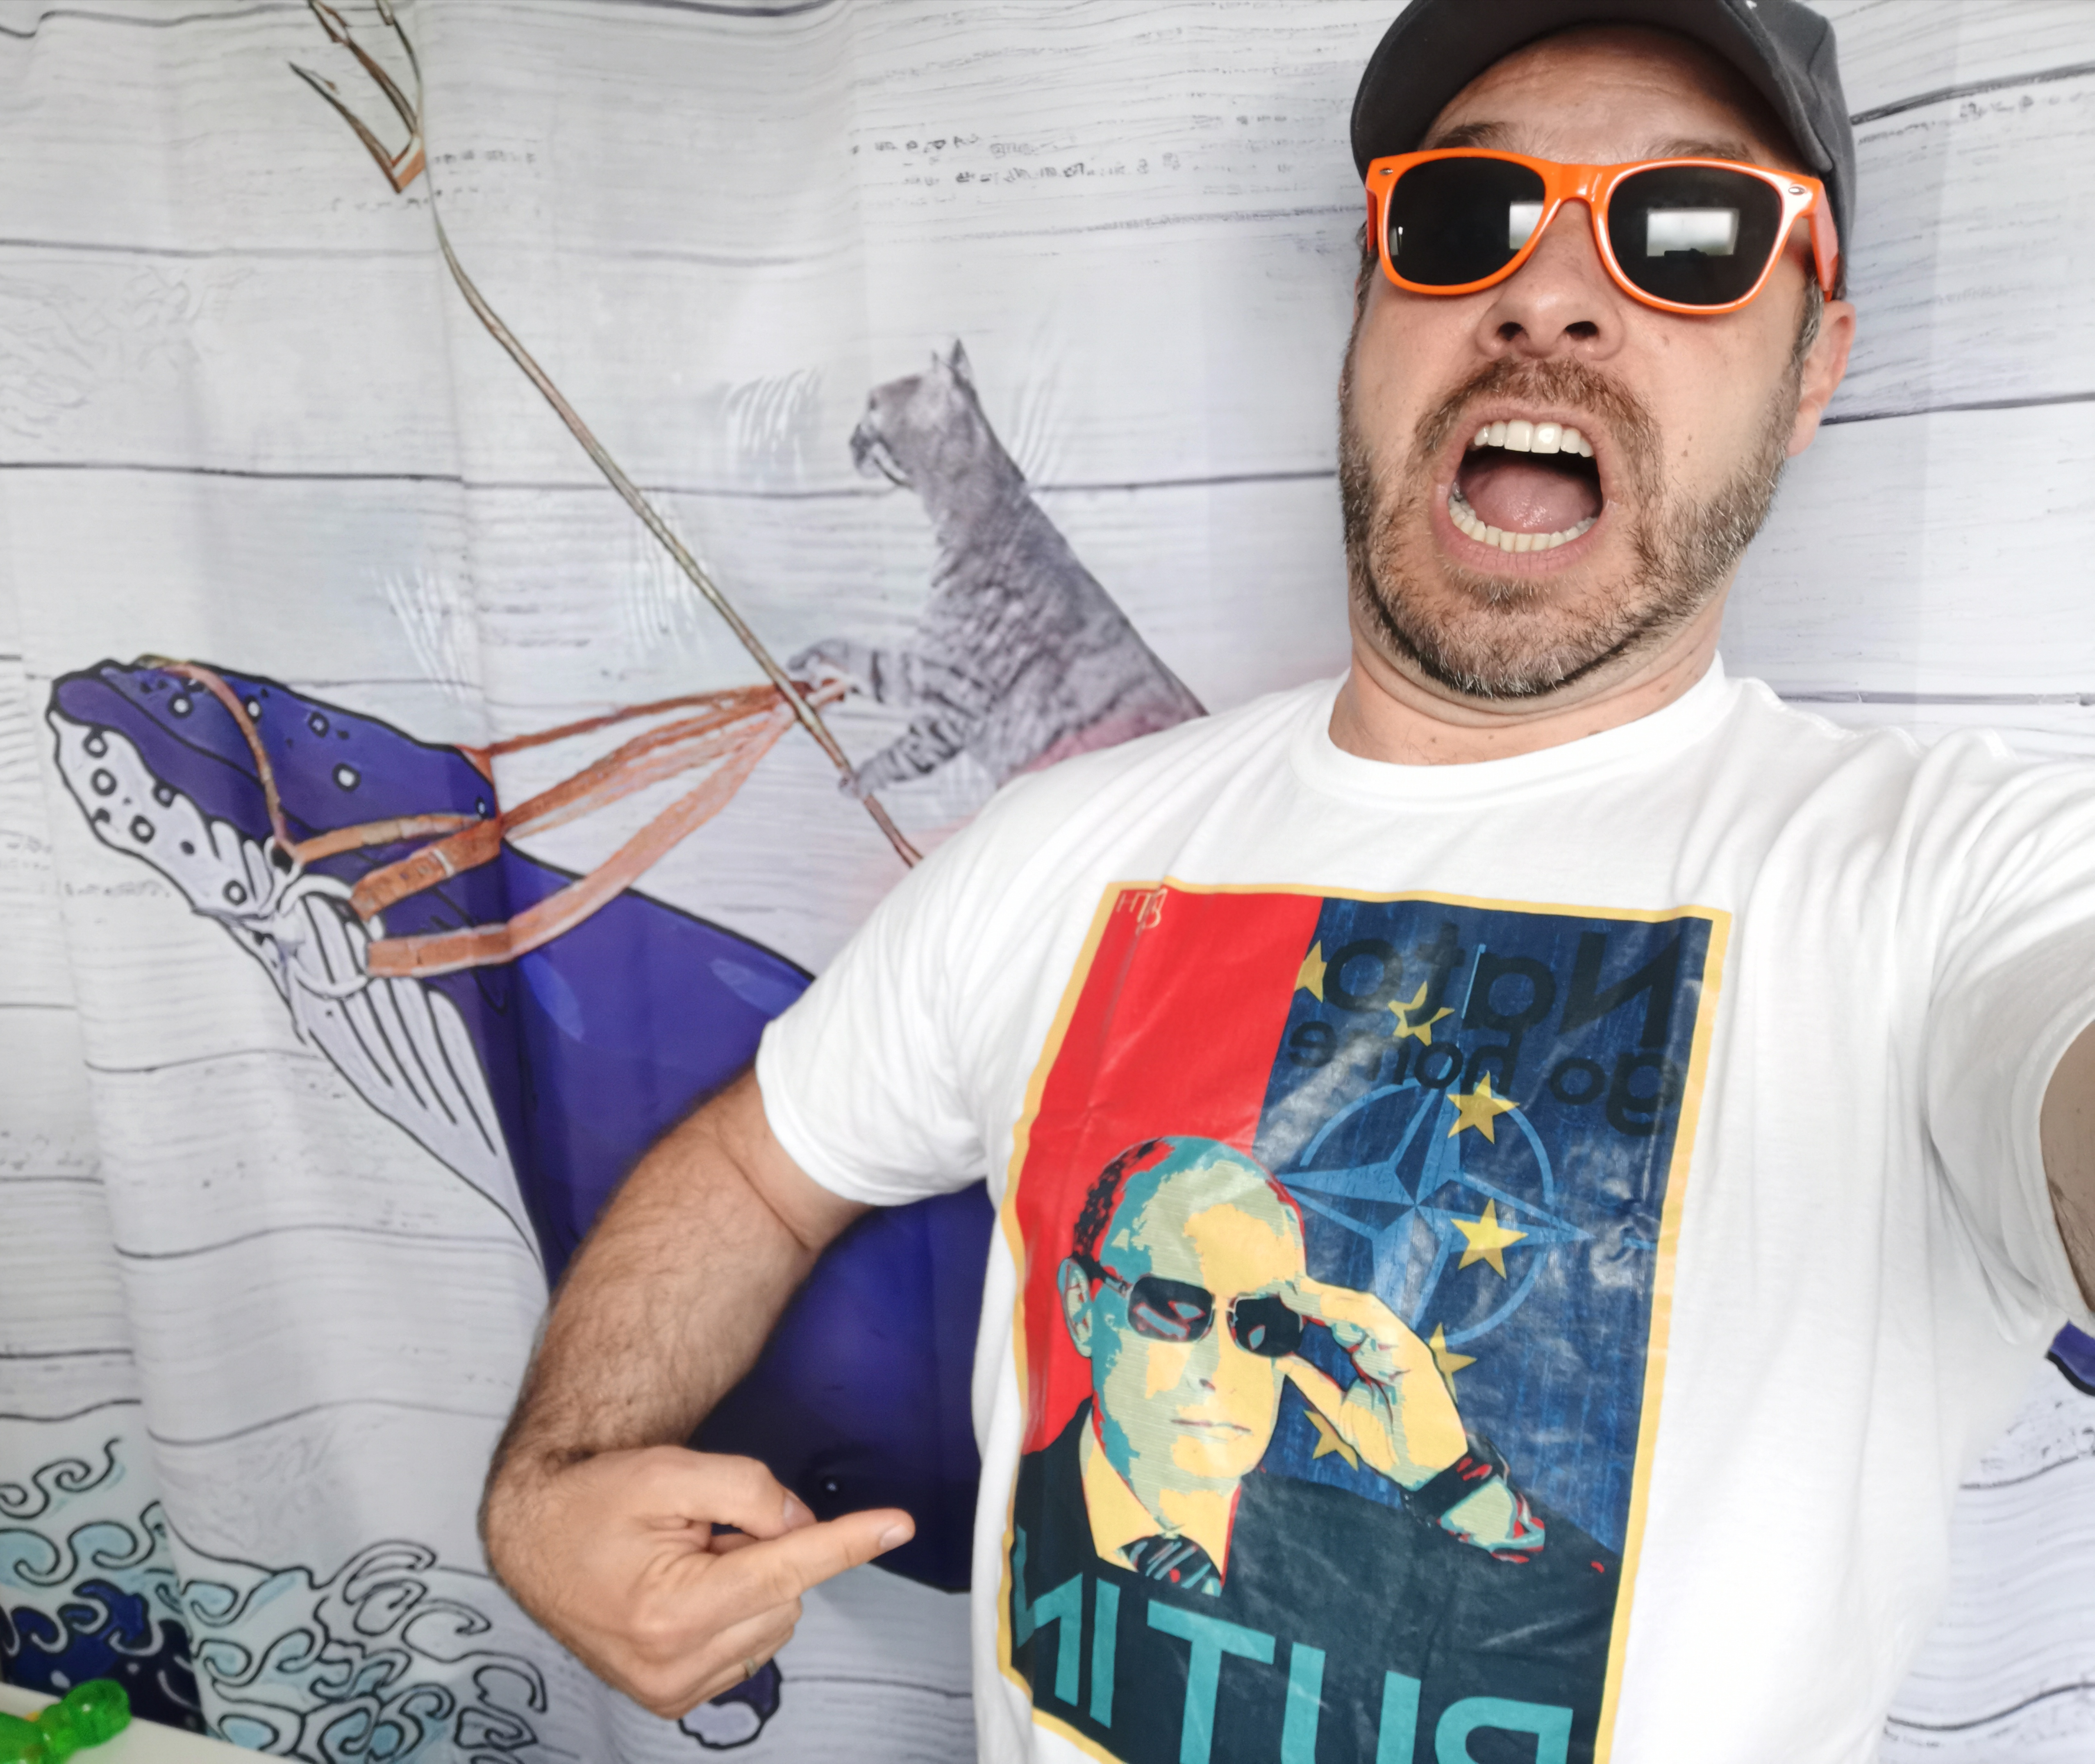
\includegraphics[width=\textwidth]{figs/fig10a}
            \caption{Image originale}
        \end{subfigure}
        \hfill
        \begin{subfigure}[b]{0.4\textwidth}
            \centering
            \includegraphics[width=\textwidth]{figs/fig10b}
            \caption{Contours}
        \end{subfigure}
           \caption{Résultats avec une photo de M. Robert, la détection est très satisfaisante ici.}
    \end{figure}
    
    \begin{figure}[h]
        \centering
        \includegraphics[width=0.7\textwidth]{figs/fig11}
        \caption{Maison carrée importée en jpg}
    \end{figure}

    On peut voir que pour cette image, le programme n’a pas fonctionné correctement. 
    En effet, l’image de base a été chargée en jpeg donc en int et non en float. 
    Ici, les nuances de gris sont représentées par des entiers et non pas par des réels entre 0 et 1 donc toutes les valeurs à 0 restent à 0 
    et les autres sont mises à 1 d’où l’excès de blanc sur l’image.
     Cette erreur amène à apprécier la régularité de l’image. Un enchaînement de 0 représente une faible variation de luminosité donc 
     une zone très régulière. Afin de contourner cette erreur, il faut donc soit changer l’image de base en png, 
     soit bouger le seuil pour pouvoir prendre en compte l’intervalle représentant les nuances de gris ( 0 à 255 ).
    

    \subsection{Dépassement}

   \subsubsection{Calcul de complexité}

    \textit{\textbf{Méthodologie de calcul :}}
    \boldmath
    \begin{itemize}
        \item On compte toutes les opérations usuelles comme $\mathcal{O}(1)$
        \item Le randint est compté en $\mathcal{O}(1)$
        \item Les chaînes étant de tailles constantes on compte le slicing comme $\mathcal{O}(1)$
        \item On calcule nos complexités avec $m$ comme variable pour la hauteur en pixel de l'image, $m$ la largeur de l'image (en pixel) et $p$ comme taille
        du masque de bruit
    \end{itemize}
    \medskip
    \textit{\textbf{Calcul :}}
    
    \begin{itemize}
        \item \textit{\textbf{image\textunderscore to\textunderscore array}} Nous utilisons du slicing sur le tableau image à la fois en largeur et en hauteur donc $\mathcal{O}(nm)$
        \item \textit{\textbf{superposition}} Seul un test est fait d'où $\mathcal{O}(1)$
        \item \textit{\textbf{calcul}} La formule de calcul est utilisée $p^2$ fois donc $\mathcal{O}(p^2)$
        \item \textit{\textbf{masque}} Dans le pire des cas, le calcul est utilisé sur tous les pixels, donc c’est en $nm\cdot C(calcul)$ d'où $\mathcal{O}(nmp^2)$
        \item \textit{\textbf{\textit{gausse}}} Seul un calcul est fait donc $\mathcal{O}(1)$
        \item \textit{\textbf{bruit}} On a une boucle en $p²$ et un appel en $\mathcal{O}(nmp^2)$ donc comme $nm >> 1$ on a donc du $\mathcal{O}(nmp^2)$
        \item \textbf{\textit{gradient}} La taille des masques est fixée à 3 d'où $\mathcal{O}(nm)$
        \item \textbf{\textit{affinage}} On applique un traitement en coût constant pour chaque pixel donc $\mathcal{O}(nm)$
        \item \textit{\textbf{voisin}} On ne teste qu’un nombre constant de valeur ( ici : 9 ) donc $\mathcal{O}(1)$
        \item \textit{\textbf{seuillage}} On applique un traitement sur tous les pixels et ensuite au pire, il n’y a que n*m pixels blanc donc la complexité de la boucle est toujours plus grande que celle du while d’où : $O(n*m)$
        \item \textit{\textbf{get}} non applicable
        \item \textit{\textbf{etape}} non applicable
    \end{itemize}
    \boldmath
    \subsubsection{Améliorations}

    Nous avons eu des difficultés pour prévoir le temps nécessaire à l'exécution des différentes fonctions et 
    particulièrement pour bruit à cause de sa complexité ( dû à sa boucle while). Nous avons donc créé d’incroyables 
    barres de progression afin de savoir si il se passe quelque chose..\newline


    Nous avons longuement réfléchi à une solution pour éviter les copier-coller lors de l’enchaînement des fonctions. 
    Nous avons donc créé les fonctions génériques get et étape qui résolvent le problème.

    \begin{figure}[h]
        \centering
        \includegraphics[width=0.9\textwidth]{figs/fig12}
        \caption{Exemple d'une barre de progression avec la durée écoulée ainsi qu'une estimation de la fin de la tâche.}
    \end{figure}

    \begin{figure}[h]
        \centering
        \includegraphics[width=0.8\textwidth]{figs/fig13}
        \caption{Code de la fonction étape \cite{git-etape} .}
    \end{figure}

    \bibliography{biblio}
    \bibliographystyle{unsrt}
    \textit{\textbf{Les sources du programme ainsi que du présent document sont accessible sur un repository github public \cite{git}}}

\end{document}